%# -*- coding: utf-8-unix -*-
\chapter{应用一:时域符号化简化模型自动生成方法}
\label{chap:time}

通过上一章的分析,可以看到电路简化模型在频率响应分析上表现出了不错的稳定性与有效性。
本章通过借用前一章分析得到的简化电路模型,尝试构造相应的电路结构,从而得到可以用于时域大信号的电路模型,并通过电路测试结果来显示方法的效果。

\section{传统的时域模型分析方法}
\label{sec:time:origin}

对于传统的运算放大器,其阶跃响应输出往往呈现如图\ref{fig:slewmeaing}所表现的形式。

\begin{figure}[!htp]
	\centering
	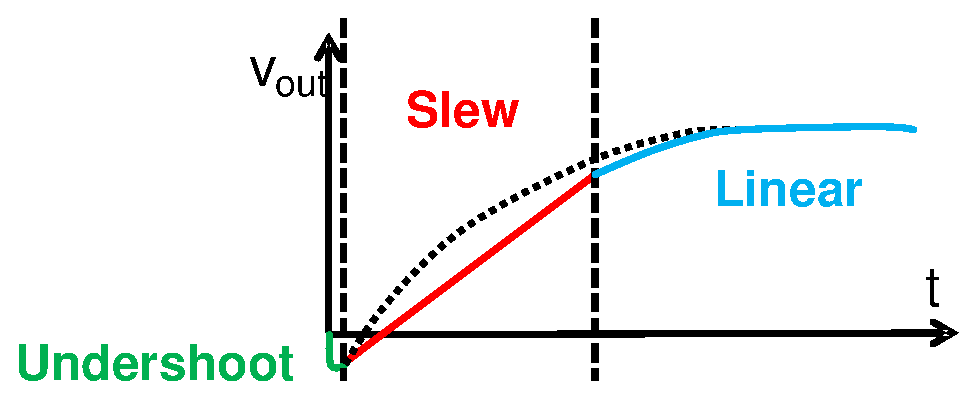
\includegraphics[width=0.6\textwidth]{chap3/SlewMeaning.eps}
	\bicaption[fig:slewmeaning]{Slew-Settling过程}{Slew-Settling过程}{Fig}{Slew-Settling procedure}
\end{figure}

图中,首先绿色部分为Undershoot部分,为线性响应,往往由于运放反馈连接中的零点造成,蓝色部分为Settling过程的线性响应部分。
其中最为关键的是红色的Slew部分。
由于在实际情况中,运放的输出能力有限,不可能输出无限大的电流,所以在运放输出端给输出端所寄生的电容充电的过程中,电压不一定能以线性的工作方式与时间呈指数上升(如黑色虚线所示)。
这种情况下由于电流输出已饱和,基本为以恒定值,故运放输出端电压随时间成比例增长,这条曲线的斜率称之为压摆率(Slew Rate,SR),一般压摆率的估计值可由输出电流$I$与输出端电容$C$的比值决定,如下式所示。

\begin{equation}
SR = \frac{I}{C}
\end{equation}

为了对运放的Slew-Settling过程进行分析,往往需要对运放的这一过程进行建模。
但是由于上述的公式十分粗糙,很难以用于比较精细的电路分析中。
故有大量研究使用各种方法对运放的时域模型进行建模。
\parencite{Pug-3Segment-2010}提出了三段式模型对这一过程进行建模。所谓三段式模型即根据运放响应的三个不同的过程(Undershoot,Slew,Settling)进行分段处理,从而形成一个用于表示运放行为的分段函数作为模型。
\parencite{Yavari-TSSlew-2005,Rezaee-FCSlew-2009}中使用了大信号分析,从电路器件模型出发,通过直接求解电路微分方程等方法对Slew-Settling行为进行分析。
这两种方式虽然有一定处理此类问题的能力,但是相对来说,其公式处理十分繁琐同时由于电路被抽象成一个个分段函数,同时往往需要计算积分等复杂运算,很难回溯会具体的电路器件进行分析,也很难自动化进行。

1982年,Chuang等人提出了在线性系统中加入限制的方式来模拟电路的Slew-Settling模型\parencite{Chuang-Slew-1982}。
这种方法因其本质上是线性系统,仅通过电流的输出能力大小来限制其输出信号,故比较适用与可以分析零极点的符号化方法。
今年来,G. Shi等人通过结合符号化零极点分析与Chuang的电路模型\parencite{ZhangHe-Slew-2011,ZhangAilin-Slew-2015},提出了使用运放宏模型的方式对运放进行建模。
这种方式不仅更为准确,同时提供了更明确的电路意义。一个二级运算放大器的电路宏模型如下图\ref{fig:macromodel}所示:

\begin{figure}[!htp]
	\centering
	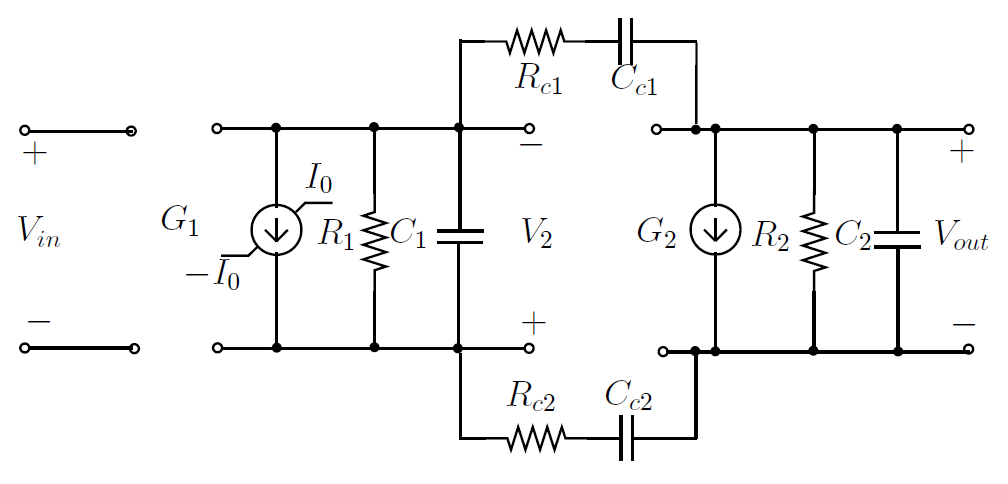
\includegraphics[width=0.6\textwidth]{chap3/macromodel.png}
	\bicaption[fig:macromodel]{运放时域宏模型}{运放时域宏模型\parencite{ZhangAilin-Slew-2015}}{Fig}{Opamp macromodel in time domain\parencite{ZhangAilin-Slew-2015}}
\end{figure}

可以看到通过提取二级运算放大器中各级的零极点,就可以得到每一级中跨导和相应的阻抗与电容。同时注意第一级运放的跨导有电流输出的限制,以模拟运放电路本身的电流输出限制。
那么现在问题就主要在于宏模型电路中各个元件的参数选取上,通过GPDD结构与模比配(Moment Matching)的方法可以得到主要的几阶项,从而得到各级的零极点关系。例如,通过GPDD计算,我们可以得到如下公式:

\begin{equation}
H\left( s \right) = \frac{{N\left( s \right)}}
{{D\left( s \right)}} = \frac{{{b_0}{s^0} + {b_1}{s^1} +  \cdots  + {b_q}{s^q}}}
{{{a_0}{s^0} + {a_1}{s^1} +  \cdots  + {a_r}{s^r}}}
\end{equation}

对上式进行泰勒展开后,可以得到:

\begin{equation}
{H_{ex}}\left( s \right) = {m_0}{s^0} + {m_1}{s^1} + {m_2}{s^2} +  \cdots
\end{equation}

其中系数可以通过联立上述两个公式后,对公式两边多次求导的方式,逐一得到相应的系数,如下式所示。

\begin{align}
& m_0 = \frac{b_0}{a_0} \nonumber \\
& m_1 = \frac{{b_1} - {m_0}{a_1}}{a_0} \nonumber \\
& m_2 = \frac{{b_2} - {m_0}{a_2} - {m_1}{a_1}}{a_0} 
\end{align}

故宏模型电路中的跨导$G$、电阻$R$和电容$C$可以以上公式计算得到。这样就建立起了宏模型与电路实际元件之间的关系,有利于日后对于电路性能优化的进一步分析。
这种方式的主要优势在于直接将电路模型中的零极点与电路元件关系挂上勾,从而电路模型不仅可以在时域,也可以在频域进行计算。
更主要的是这种模型,传统仿真器中可以简单地通过编写网表得到,仿真方便便捷。

\section{符号化时域简化模型分析方法}
\label{sec:time:simp}

\subsection{时域符号化简化流程}
\label{subsec:time:simp:process}

本方法的基本流程类似于Chuang模型,首先获取简化的小信号模型,然后在该小信号模型的基础上加入对输出电流饱和的限制。
但是,本方法与Chuang模型有三点不同,分别为:

\begin{enumerate}[label=\emph{\alph*})]
	\item 简化的小信号零极点模型可以直接通过第二章的符号化模型降阶算法得到。
	\item 限制电流加载运放中所有得以保留的$g_m$元件上,并用大信号中的通过管子的电流作为其限制电流。
	\item 采用了更加光滑的非线性函数,以更加真实地模拟实际情况。
\end{enumerate}

\begin{figure}[!htp]
	\centering
	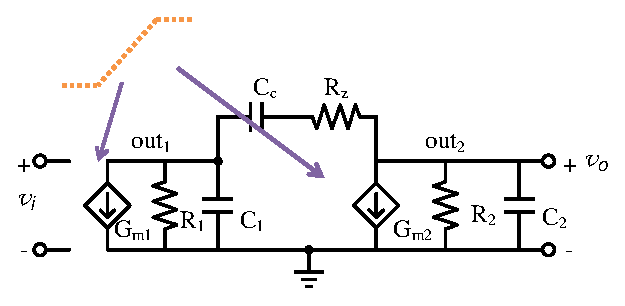
\includegraphics[width=0.6\textwidth]{chap3/CurrentLimitPos.eps}
	\bicaption[fig:limitcur]{时域模型中的电流限制位置}{时域模型中的电流限制位置}{Fig}{Current limit position in slew-settling model}
\end{figure}

其中第一点正是相比之前的方法的闪光点。因为之前的方法,即使是一般的零极点模型,往往很难建立模型与电路元件之间的关系,而给出简化小信号模型可以直观地给出两者之间的联系。

第二点可参考图\ref{fig:limitcur}的示意,本方法将运放电路中所有存在的$g_m$均加入限制。
\parencite{Yavari-TSSlew-2005}中指出,现代的模拟集成电路由于其功耗降低,电源电压降低等原因,造成电流输出饱和的原因不一定是由输入级决定的,可能是之后的电路充电速度不足导致。
Chuang模型中只考虑了第一级电路的输出饱和,对之后级的输出限制没有做出过多考量。
如果在各个$g_m$上加入相应的电流限制,那么即可模拟各级中的电流限制。

\begin{figure}[!htp]
	\centering
	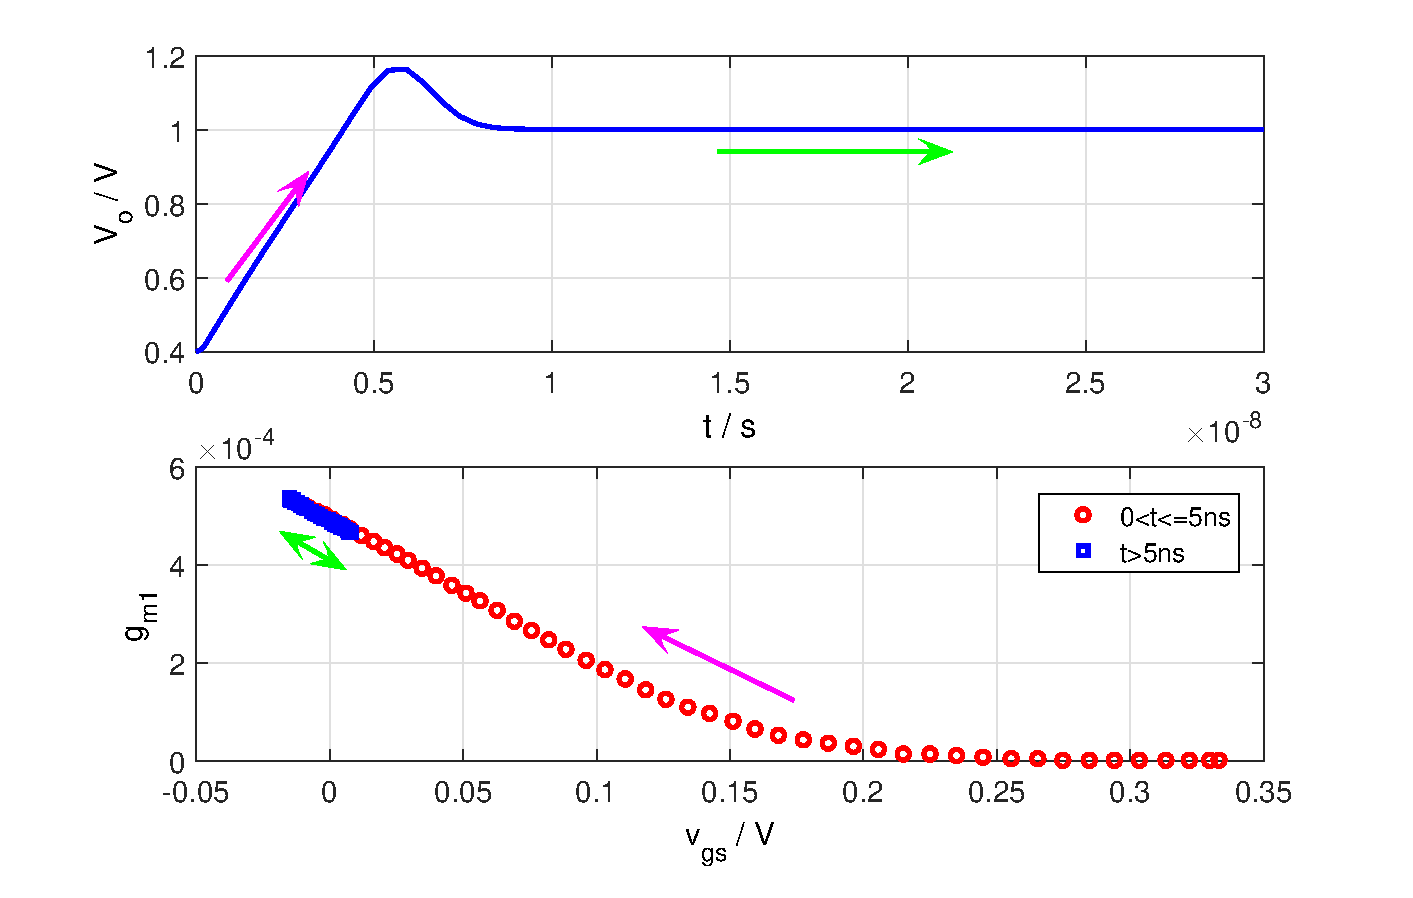
\includegraphics[width=0.8\textwidth]{chap3/gmvariation.eps}
	\bicaption[fig:gmvariation]{Slew-settling过程中输入管$g_m$的变化}{Slew-settling过程中输入管$g_m$的变化}{Fig}{$g_m$ variation during the slew-settling procedure}
\end{figure}

图\ref{fig:gmvariation}给出了两级运算放大器slew-settling的过程中输入管的$g_m$随着输入交流小信号的变化。
图中箭头方向代表了时间的流向。在Slew过程(红色圆圈)中,$g_m$快速爬升至所需要的稳态情况的值;而在Settling过程(蓝色方块)中,$g_m$稳定在某一值不再变化。
以往,我们往往假设$g_m$的函数是一个分段函数,在未饱和前,输入电压和输出电流成正比;饱和后,输出稳定电流。
这样的话$g_m$仅有两个值,其一是稳态情况下的跨导,另一个是$0$。
然而在图中明显看到这样的假设是不合理的,一个办法就是重新决定施加给$g_m$的非线性函数。

\subsection{非线性函数选取}
\label{subsec:time:simp:nonlinear}

非线性函数有许多不同的形式。
一类合适的函数是S型函数族$S_i\left(x\right)$。
这里列举了五种不同的函数方程共参考:
\begin{align}
&{S_0}\left( x \right) = \left\{ {\begin{array}{*{20}{c}}1 & {x \geqslant 1}  \\x & { - 1 \leqslant x < 1}  \\{ - 1} & {x < 1}  \\\end{array} } \right. \\
&{S_1}\left( x \right) = \tanh \left( x \right) \hfill \\
&{S_2}\left( x \right) = \frac{2}{\pi }gd\left( {\frac{\pi }	{2}x} \right) = \frac{2}{\pi }\arcsin \left( {\tanh \left( {\frac{\pi }{2}x} \right)} \right)\\
&{S_3}\left( x \right) = \frac{x}{{\sqrt {1 + {x^2}} }}\\
&{S_4}\left( x \right) = \frac{2}{\pi }\arctan \left( {\frac{\pi }{2}x} \right)
\end{align}

\begin{figure}[!htp]
	\centering
	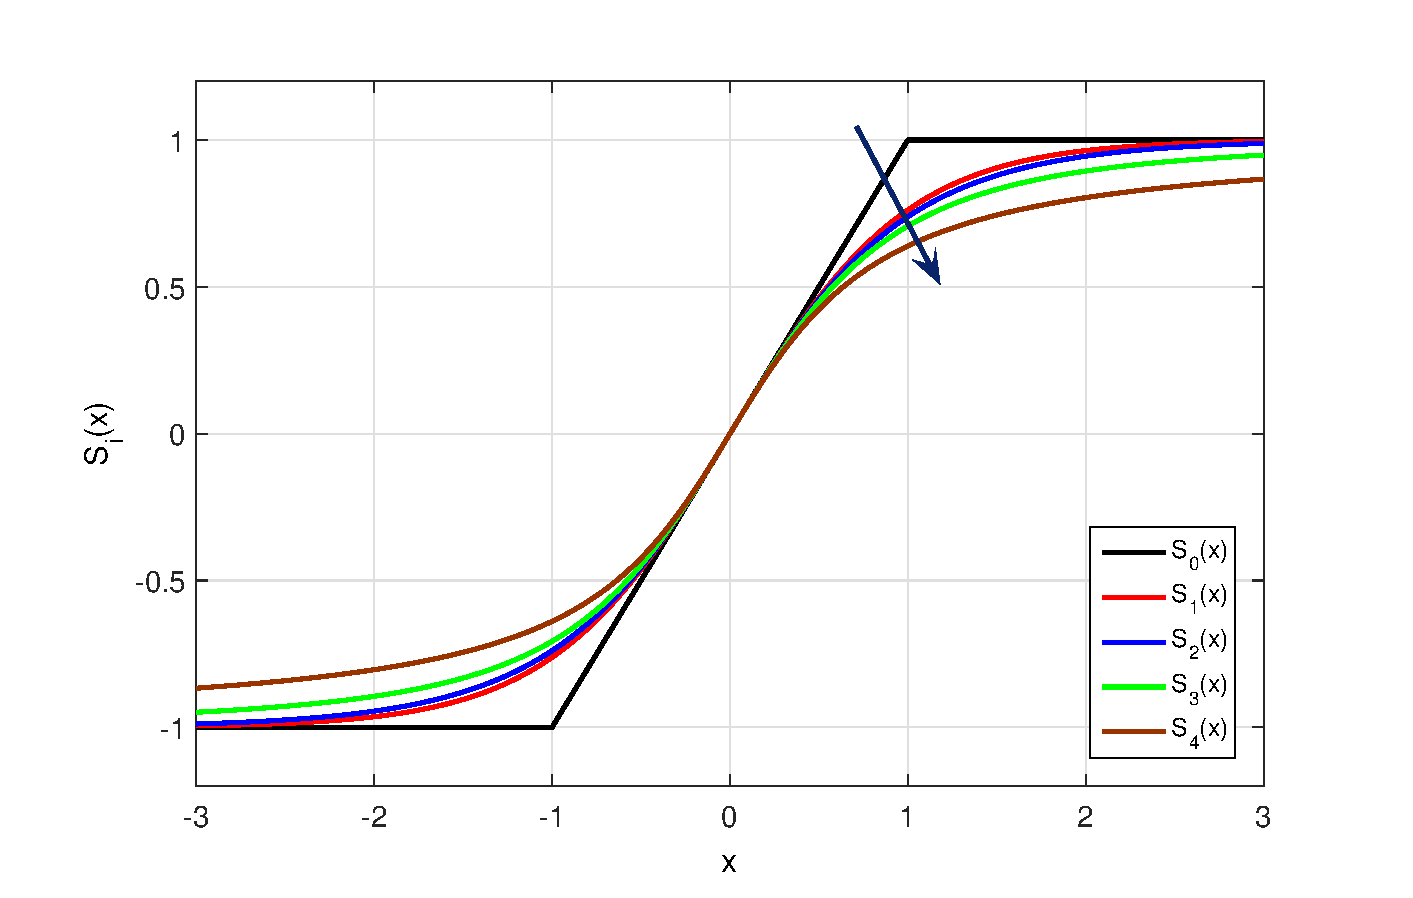
\includegraphics[width=0.8\textwidth]{chap3/sigmoid.eps}
	\bicaption[fig:sigmoid]{S型函数族}{S型函数族}{Fig}{Sigmoid function family}
\end{figure}

图\ref{fig:sigmoid}中展示了所有这5中S型函数的曲线。
可以看到原先在Chuang模型中使用的非线性函数即为这里的$S_0\left(x\right)$。
图中的箭头显示了这些函数在正半平面或负平面中不互相相较,且呈现出了一定顺序。
这类函数有一些共同的特征,如它们都绝对单调递增,可总结如下:

\begin{eqnarray}
\mathop {\lim }\limits_{x \to  + \infty } {S_i}\left( x \right) = 1\\
\mathop {\lim }\limits_{x \to  - \infty } {S_i}\left( x \right) = -1\\
{\left. {\frac{d}{{dx}}{S_i}\left( x \right)} \right|_{x = 0}} = 1
\end{eqnarray}

如果有一个跨导的DC偏置电流是$I_0$,其增益为$g_m$,那么对这类函数只需要做如下的变换即可得到我们所需要的非线性的$g_m$。

\begin{equation}
{I_0}{S_i}\left( {\frac{{{g_m}}}{{{I_0}}}x} \right)
\end{equation}

\section{符号化时域简化模型分析方法}
\label{sec:time:test}

\subsection{两级运放测试结果}
\label{subsec:time:test:ts}

\begin{figure}[!htp]
	\centering
	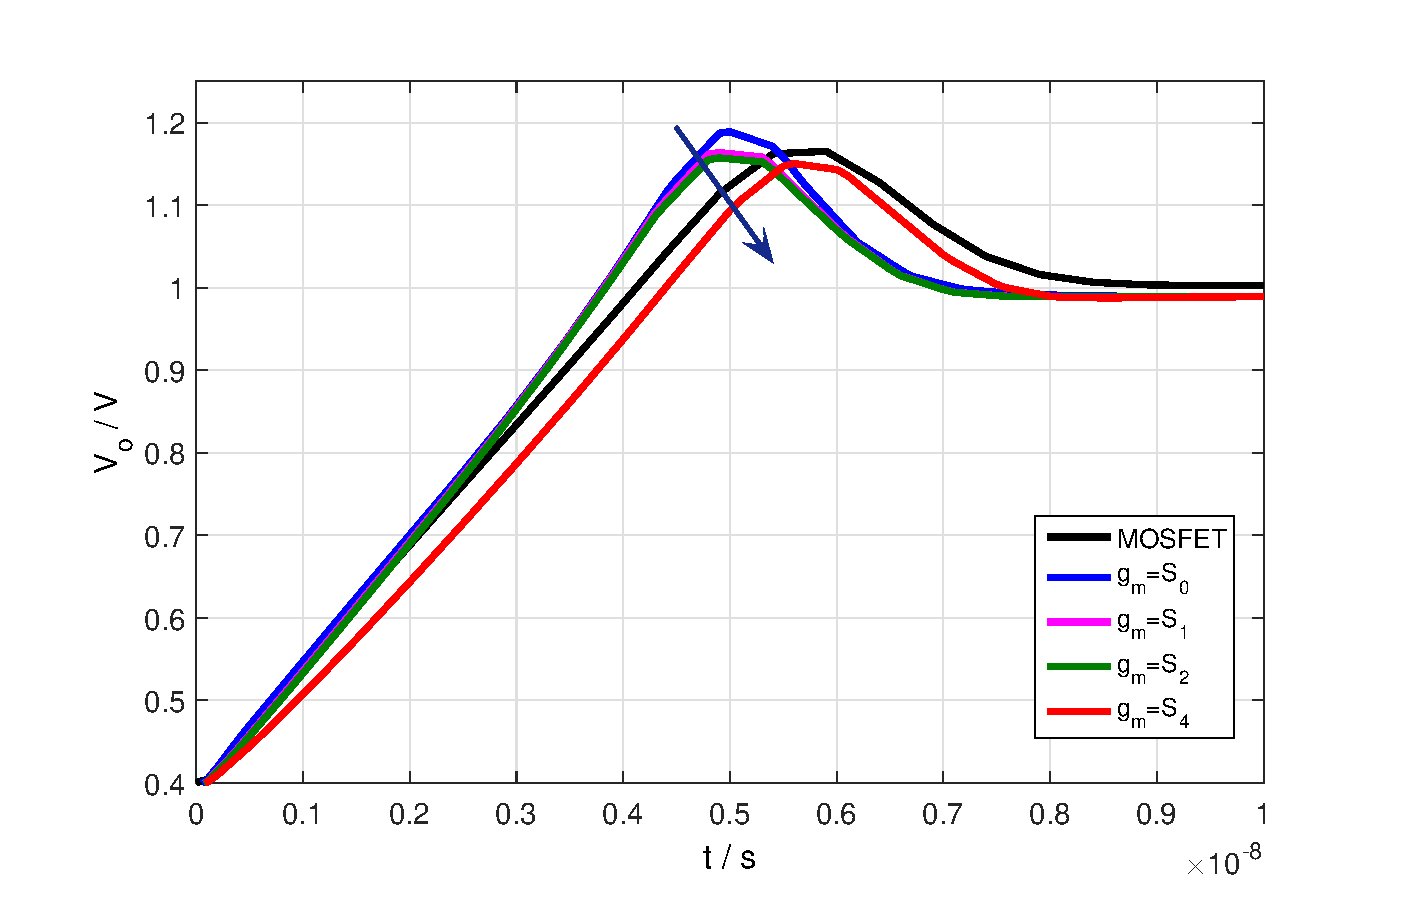
\includegraphics[width=0.8\textwidth]{chap3/TS_Slew.eps}
	\bicaption[fig:tsslew]{两级运放模型的Slew-Settling时域仿真结果}{两级运放模型的Slew-Settling时域仿真结果}{Fig}{Simulation Results of slew-settling behavior for two-stage opamp model}
\end{figure}

首先我们针对两级运放电路进行了电路时域模型的建模,图\ref{fig:tsslew}中展示了在不同S型函数作用下的电路的Slew-Settling行为。
可以看到$S_0\left(x\right)$、$S_1\left(x\right)$和$S_2\left(x\right)$在Slew阶段表现出了良好的对压摆率的估计行为。
而$S_4\left(x\right)$则非常适于对于电路稳定时间的估计。
这里并没有画出相应的$S_3\left(x\right)$的曲线,因为其HSPICE仿真并不收敛。
可以发现图中的箭头标志了这些函数作用下的时域曲线也呈现了一定的顺序,且与上一小节中的次序一致。
故可以预估$S_3\left(x\right)$会取得最好的电路近似程度。

\subsection{折叠共源共栅运放测试结果}
\label{subsec:time:test:fc}

在对折叠共源共栅运放的电路测试中,我们发现只有$S_1\left(x\right)$的作用下,电路才可以顺利由HSPICE求解出来,仿真结果如图\ref{fig:fcslew}。
这里结果十分值得怀疑,因为其中出现了奇怪的折角,这在电路稳定的情况下不应该出现。
同时,此时本方法生成的时域运放模型并不能很好地抓取电路的时域特性,说明时域模型生成方法仍存在一些问题,需要进一步分析验证。

\begin{figure}[!htp]
	\centering
	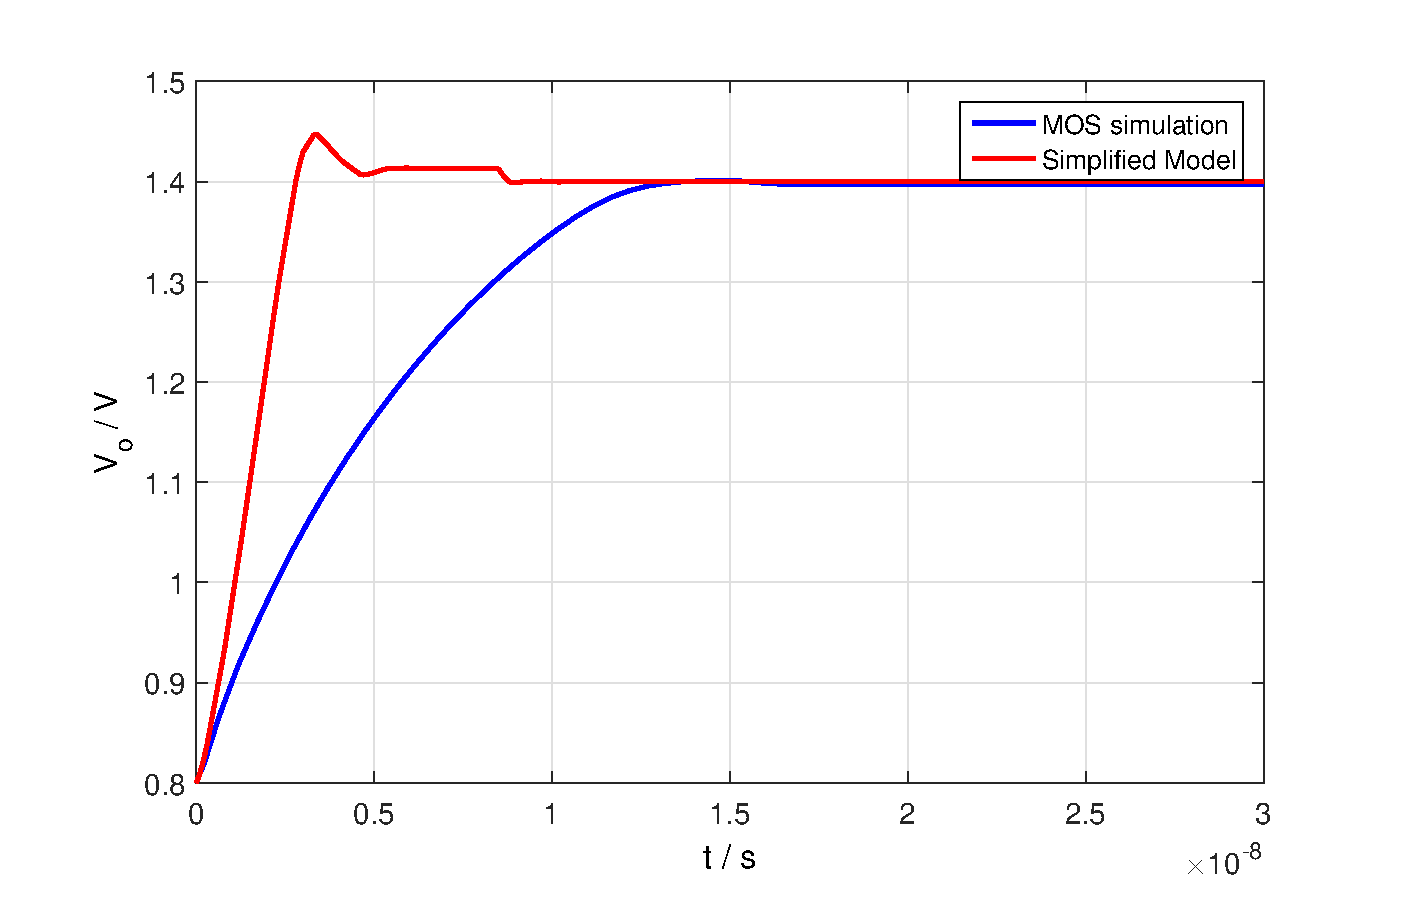
\includegraphics[width=0.8\textwidth]{chap3/FC_Slew.eps}
	\bicaption[fig:fcslew]{折叠共源共栅运放模型的Slew-Settling时域仿真结果}{折叠共源共栅运放模型的Slew-Settling时域仿真结果}{Fig}{Simulation Results of slew-settling behavior for folded-cascode opamp model}
\end{figure}

\section{本章小结}
\label{sec:time:con}

本章主要回顾了时域模型生成方法的相关历史,并提出了自己的时域模型简化方法,并对方法进行了测试。
这种方法的优势在于其生成的模型是符号化的,并且大部分流程可以自动化,不需要过多的电路经验也可以对电路模型进行分析。
可以看到目前符号化时域简化模型分析方法仅针对部分电路可以成功使用,但是仍有许多电路存在分析困难的情况。
需要进一步通过非线性函数选取和系统层面理论分析对电路模型生成的方法进行论证。